\subsection{Bunch-by-bunch}
This is essentially a \textbf{correction} system, but it could be used for \textbf{measurement} too.

The oscillations that the bunch-by-bunch (BbB) system wants to correct are the coherent coupled bunch oscillations. In this type of oscillation, all bunches oscillates with same amplitude and frequency. The only thing that can vary from one bunch to another is the phase of their oscillation, but the phase difference between any two consecutive bunches remains constant. This phase difference is described as
\begin{equation}
	\Delta \varphi = m \frac{2\pi}{M}
\end{equation}
where $M$ is the number of bunches and $m$ is an integer between 0 and $M-1$ called eigenmode.

Although the physical explanation about how coherent coupled bunch oscillations occurs it's not the focus here, it's sufficient to say that this type of instability is "excited by the interaction of the particle beam with its surroundings" \cite{lonza}, and this interaction can excite different eigenmodes at the same time. In any case, the phase difference $\Delta \varphi$ remains constant.

\begin{itemize}
	\item Both two transversal planes and longitudinal plane are affected by those oscillations. Therefore, the BbB system acts over all of them.
\end{itemize}

Differently from the spectrum analyzer system, the BbB system doesn't need to excite the beam. It's already excited by the coherent coupled bunch oscillations. So only a measurement and a correction process are necessary.

The measurement process starts with a BPM. All its four antennas are used, and their signals are carried out to an analogue system called monopulse. The monopulse process these four signals and turn them into three outputs: $x$, $y$ and $z$ which, for a configuration like the one shown in \autoref{fig:BPMsketch}, are essentially given by
\begin{align}
	x = \frac{A+D-B-C}{z}\\
	y = \frac{A+B-C-D}{z}\\
	z = A+B+C+D
\end{align}
where $A$, $B$, $C$ and $D$ are the signals received from antennas A, B, C and D, respectively. A more detailed explanation about how this position calculation is done could be find in \cite{digBPMCalculation}.

\begin{figure}[!htb]
	\centering
	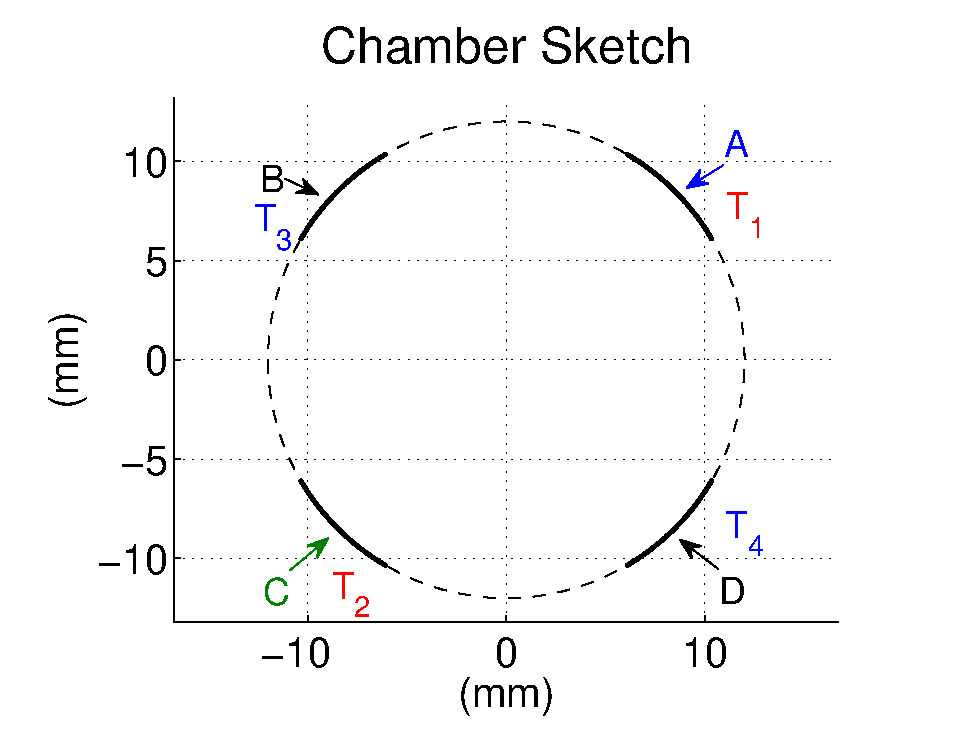
\includegraphics[width=0.7\linewidth]{./Figures/BPMsketch.eps}
	\caption{Vacuum chamber illustration showing BPM antennas position. Reprinted from \cite{digBPMCalculation}.}
	\label{fig:BPMsketch}
\end{figure}

Then, these three analogue signals go to a demodulator unit called front-end which "receives the position error signals modulated around the third harmonic, provides gain and proceeds with analog down-conversion" \cite{digBPMCalculation}. Roughly speaking, it prepares those signals so they could be used on the next BbB system stages.

Proceeding, all front-end outputs go to the processing unit, the core of the BbB system. It receives those signals and split them to various processors, one for each bunch. In that way, each processor can work independently with its respective bunch signal and all bunches signals are processed simultaneously. In this process, all the actuator signal calculus is done. In a few words, when the BbB system starts, the processor waits until it has enough samples to compute a wave signal that models the original one. When it does, since the oscillation frequency is almost constant, it could generate an opposite signal (one with a phase difference of 180 degrees) to correct the oscillation just by waiting the exact time the original signal takes to advance its phase in 180 degrees. Doing that spares the processor from generating an opposite wave signal, which would cost some important processing time. Finally, it brings all bunches signals together to compute its output.

\begin{itemize}
	\item The number of samples needed to model the original signal is defined by the number of taps of the output FIR filter. Those samples fill a buffer used to compute the actuator signal. This buffer starts empty and, as the samples are arriving, it substitutes the last sample for the new one. So, after this minimum number of samples is achieved, the measurement is always computed with the newest samples.
\end{itemize}

At UVX, "the transverse system implemented (...) is based on Instrumentation Technologies processors. Dimtel's iGP processor for controlling longitudinal instabilities were also evaluate at UVX storage ring" \cite{digFeedback}.

After the processing stage, the signal pass through an amplifier and goes to the control system actuator, which is a stripline kicker for both transverse systems and a longitudinal kicker (overloaded cavity) for the longitudinal one.

\begin{itemize}
	\item An amplifier is needed because the signal from the processing unit has not enough power to excite the beam.
\end{itemize}

\autoref{fig:BbBdiagram} presents a general topology of the BbB system.

\begin{figure}[!htb]
	\centering
	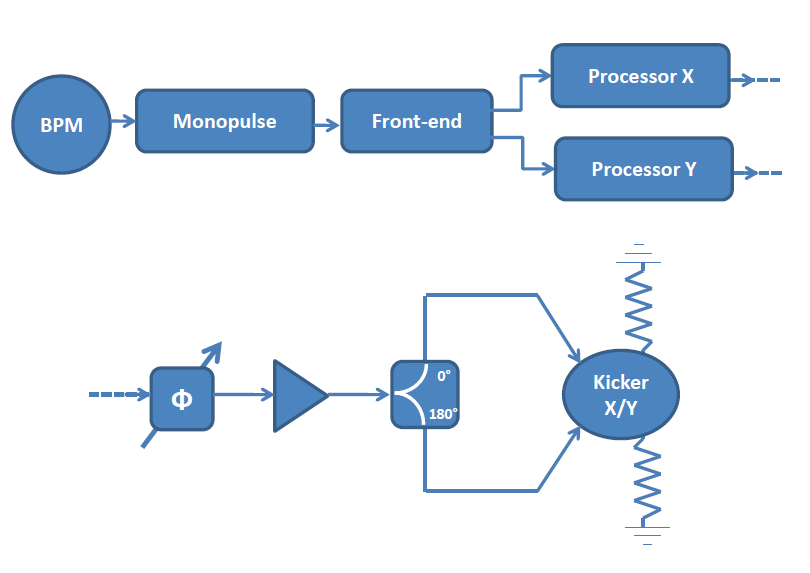
\includegraphics[width=0.8\linewidth]{./Figures/BbBdiagram.png}
	\caption{Bunch-by-bunch feedback system general topology. Reprinted from \cite{digFeedback}.}
	\label{fig:BbBdiagram}
\end{figure}

To turn this into a measurement system, it's possible to modified the BbB system so its output be in phase with the original signal. This would change the configuration of the control loop from a negative feedback to a positive one, exciting the beam instead of damping its oscillation. Then it's only necessary to convert the signal from time domain to frequency with a Fast Fourier Transform (FFT). Fortunately, each bunch is processed separately and one bunch is sufficient for measuring the tunes. So the BbB system could be configured to work with one bunch in positive feedback and the others in negative feedback, measuring the tunes and still correcting the coherent coupled bunch oscillations.

\subsubsection{Notes}
There are some important differences between signal analyzer and BbB systems that should be emphasized.

First, the signal analyzer system works in frequency domain, while the BbB works in time. Frequency domain analysis are characterized for its high sensitivity and slow response. On the other hand, time domain analysis are exactly the opposite: characterized by low sensitivity and fast response. So, if something with little and periodic variation needs to be observed, a frequency domain system is more suitable. But if it's something with big and momentary variation instead, a time domain system is required. Which are exactly the cases of the signal analyzer and BbB systems, respectively.

Second, when the BbB system is operating with one bunch in positive feedback, a common question would be if this affects the beam stability or something else. The answer is no. When only one bunch is outside the control loop, neither the beam stability or the machine emittance are significantly affected.

\pagebreak